% Template for NIME 2014
%
% Modified by Baptiste Caramiaux on 25 November 2013
% Modified by Kyogu Lee on 7 October 2012
% Modified by Georg Essl on 7 November 2011
%
% Based on "sig-alternate.tex" V1.9 April 2009
% This file should be compiled with "nime2011.cls"
%

\documentclass{nime-alternate}

\usepackage{fixltx2e}
\usepackage{float}
\usepackage{url}

\begin{document}
%
% --- Author Metadata here ---
\conferenceinfo{NIME'14,}{June 30 -- July 03, 2014, Goldsmiths, University of London, UK.}

\title{Auraglyph}
\subtitle{Handwritten Computer Music Composition and Design}

%
% You need the command \numberofauthors to handle the 'placement
% and alignment' of the authors beneath the title.
%
% For aesthetic reasons, we recommend 'three authors at a time'
% i.e. three 'name/affiliation blocks' be placed beneath the title.
%
% NOTE: You are NOT restricted in how many 'rows' of
% "name/affiliations" may appear. We just ask that you restrict
% the number of 'columns' to three.
%
% Because of the available 'opening page real-estate'
% we ask you to refrain from putting more than six authors
% (two rows with three columns) beneath the article title.
% More than six makes the first-page appear very cluttered indeed.
%
% Use the \alignauthor commands to handle the names
% and affiliations for an 'aesthetic maximum' of six authors.
% Add names, affiliations, addresses for
% the seventh etc. author(s) as the argument for the
% \additionalauthors command.
% These 'additional authors' will be output/set for you
% without further effort on your part as the last section in
% the body of your article BEFORE References or any Appendices.

\numberofauthors{2}

\author{
%% 1st. author
%\alignauthor
%Spencer Salazar\\
%       \email{spencer@ccrma.stanford.edu}
%% 2nd. author
%\alignauthor
%Ge Wang\\
%       \email{ge@ccrma.stanford.edu}
%\and
%       \affaddr{Center for Computer Research in Music and Acoustics (CCRMA)}\\
%       \affaddr{Stanford University}\\
%       \affaddr{Stanford, CA  94305}
\alignauthor
First Author\\
       \email{author@example.com}
% 2nd. author
\alignauthor
Second Author\\
       \email{author@example.com}
\and
       \affaddr{Department}\\
       \affaddr{University}\\
       \affaddr{City, Region, Postal Code, Country}
}

\teaser{
	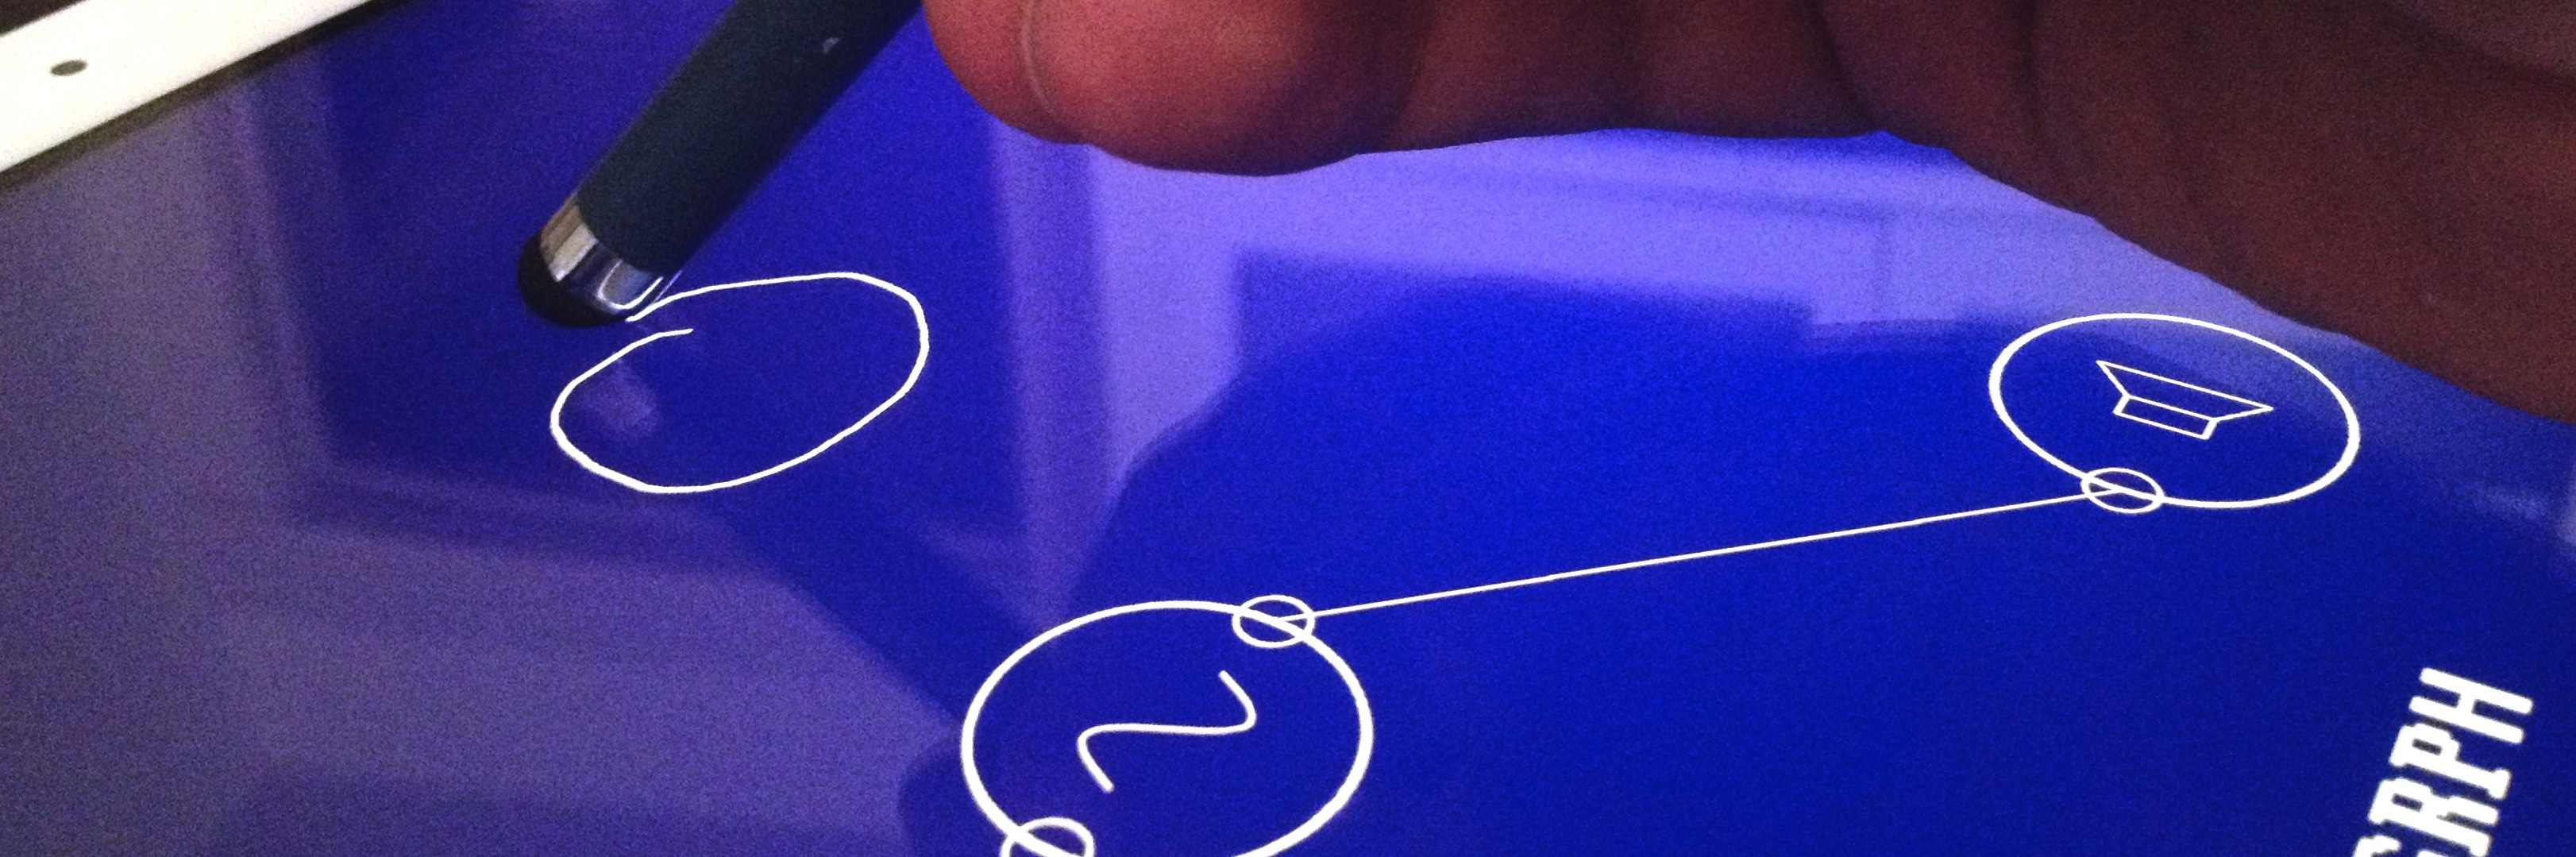
\includegraphics[width=1\textwidth]{figures/auragraphHand.jpg}
	\caption{Auraglyph in use.}
	\label{fig:auraglyphInUse}
}

\date{31 January 2014}

\maketitle

\begin{abstract}

Effective software interaction design must consider all of the capabilities and limitations of the platform for which it is developed. 
To this end, we propose a new model for computer music system design on touchscreen devices, combining both pen/stylus input and multitouch gestures. 
Such a model surpasses the barrier of touchscreen-based keyboard input, preserving the primary interaction of touch and direct manipulation throughout the development of a complex musical program. 
We have implemented an iPad software application utilizing these principles, called ``Auraglyph.''
Auraglyph offers a number of fundamental audio processing and control operators, as well as facilities for structured input and output, all which may be created, parameterized, and interconnected via stylus and touch input. 
Underlying this application is an advanced handwriting recognition framework, LipiTk, which can be trained to recognize both alphanumeric characters and arbitrary figures, shapes, and patterns. 

\end{abstract}

\keywords{computer music systems, handwriting recognition, touchscreen, multitouch input}

\section{Introduction}
\label{sec:Introduction}

Touch-based computing has profoundly altered the landscape of mainstream computing in the early 21st century. 
Since the introduction of the iPhone in 2007, and later the iPad in 2010, scores of touchscreen devices have entered the popular consciousness, from mobile phones, tablet computers, watches, and desktop computer screens, to name a few. 
New human-computer interaction paradigms have accompanied these hardware developments, addressing the complex shift from classical keyboard-and-pointer computing to multitouch interaction. 
We propose a new model for touchscreen interaction with musical systems: the combined use of stylus-based handwriting input and direct touch manipulation. 
This system provides a number of advantages over existing touchscreen paradigms for music. 
Stylus input, complemented by machine learning-based handwriting recognition, provides a number of advantages in this scheme. 
Firstly, it replaces the traditional role of keyboard-based text/numeric entry with handwritten letters and numerals.
It additionally allows for modal entry of generic shapes and glyphs, for example, canonical oscillator patterns (sine wave, sawtooth wave, square wave, etc.) or other abstract symbols.
Finally, the stylus provides precise graphical free-form input for e.g. filter transfer functions, envelopes, and parameter automation curves. 
Multitouch finger input continues to provide functionality that has become expected of touch-based software, such as direct movement of on-screen objects, interaction with conventional controls (sliders, buttons, etc.), and other manipulations. 
Herein we discuss the design, prototyping, and evaluation of one implementation of such a system, which we have titled ``Auraglyph.''

\begin{figure*}[h!]
	\centering
		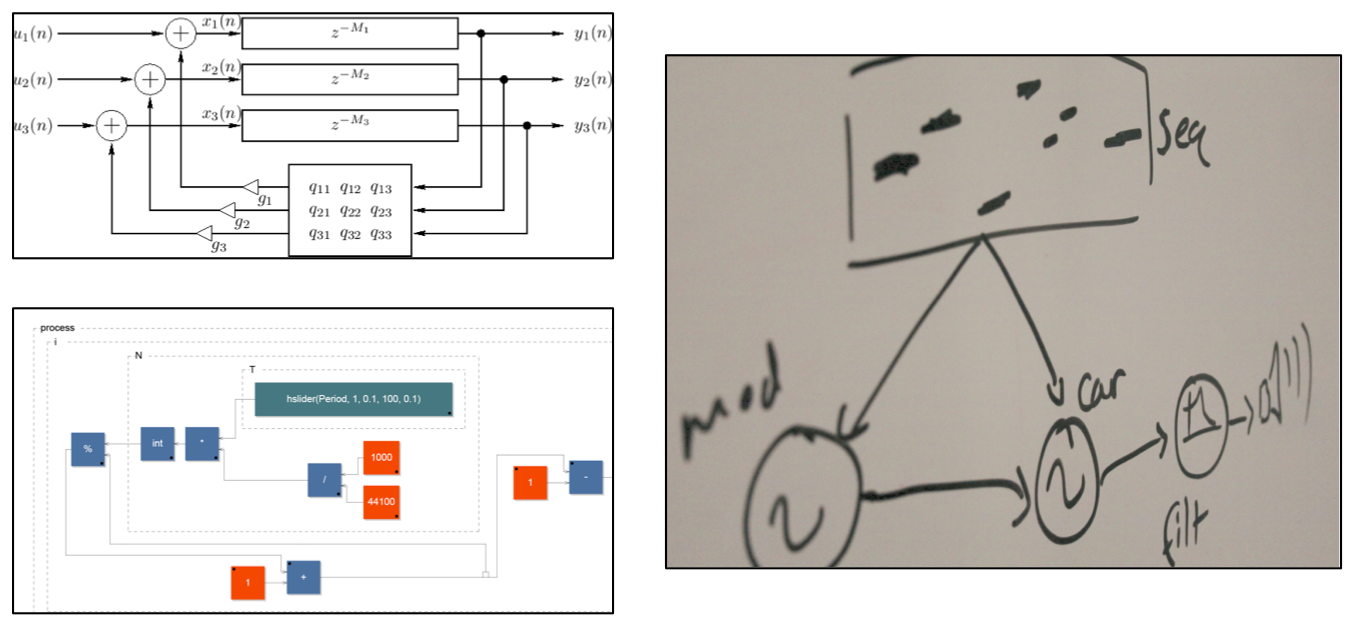
\includegraphics[width=0.9\textwidth]{figures/block.png}
	\caption{Example block diagrams. Top-left: a feedback delay network\protect~\cite{smith2010pasp}. Bottom-left: compiler-generated block diagram from the Faust programming language\protect~\cite{faustOnline}. Right: hand-drawn block diagram.}
	\label{fig:blockDiagram}
\end{figure*}

\section{Related Work}
\label{sec:RelatedWork}

%Touchscreens and music: 
%Handwriting recognition and music: "Exemplar-based learning in adaptive optical music recognition system" (Fujinaga 1996)

In our research, handwriting recognition has previously found little use in interactive computer music. 
Fujinaga et al. explored character recognition of traditional staved musical notation~\cite{fujinaga1989computer, fujinaga1996exemplar}, as have Miyao and Marayuma~\cite{miyao2007online}. 
Direct, graphical manipulation of computational data via pen or stylus, augmented by computer intelligence, goes back as far as Sutherland's Sketchpad~\cite{sutherland1964sketch} and GRAIL and the RAND Tablet by Ellis et al.~\cite{davis1964rand}. 

Object graph-based programming languages such as Puredata~\cite{puckette1996pure} and Max/MSP~\cite{zicarelli1998extensible} have tremendously influenced the space of visual computer music design and composition. 
More recently, Kronos extended functional programming models to a visual space in the context of real-time music performance~\cite{norilo2012visualization}. 
Mira dynamically replicates the interface of desktop-based Max/MSP programs on a tablet, joining conventional music software development with touch interaction~\cite{tarakajian2013anmira}. 

%Various iPad (Magic Fiddle)

%
%Interaction design: 
%

\section{Handwritten Computer Music}
\label{sec:HandwrittenComputerMusic}

This work has been motivated by a desire to better understand the distinguishing capabilities and limitations of touchscreen technology, and, using these as guiding principles, to enable expressive music interactions on such devices. 
Complex software developed for a given interaction model -- such as keyboard-and-mouse -- may not successfully cross over to a different interaction model -- such as a touchscreen device. 
In these regards, much inspiration was drawn from a number of products by mobile software developer Smule, including Ocarina~\cite{wang2014ocarina}, whose properties as a musical instrument and experience were designed for the specific affordances of the iPhone. 
While a conventional laptop computer has many of the same features as an iPhone (buttons, microphone, speakers, and in some cases multitouch screen), it is barely conceivable that Ocarina could function on a laptop\footnote{As a software engineer in the development of Ocarina, I had the privilege of running a development version of Ocarina on a laptop-based iPhone simulator. Despite the comedy of playing music by blowing into the laptop's microphone, located to the left of the keyboard, this experience left much to be desired with respect to interaction.}.

The initial insight leading to this work was that numeric and text input on a touchscreen might be more effectively handled by recognizing hand-drawn numerals and letters, rather than an on-screen keyboard. 
We soon realized that we could use handwriting recognition to analyze a substantial number of handwritten figures and objects beyond just letters and numbers. 
A user could then draw entire object graphs and audio topologies, to be realized as an audio system or musical composition, in real-time, by the underlying software application. 

From here a natural metaphor for interaction arose, that of a handwritten block diagram.
Block diagrams, both computer-generated and manually produced, are utilized extensively in digital audio and computer music development processes (Figure \ref{fig:blockDiagram}). 
We would like users of our system to think that they are drawing a block diagram of their musical system on a whiteboard or sheet of paper, and then to have that design made manifest. 

This metaphor provides several notable benefits. 
Writing and drawing with a pen or pencil on a flat surface is a foundational interaction for an incredible number of individuals, as this activity is developed from early education around the world. 
Moreoever, a common goal, perhaps the ultimate goal, of computer interfaces is to simplify the mapping between the user's conceptual abstraction of an idea and translating that idea to a digital representation. 
The extent to which this goal is met determines the ease of a user successfully inputting their data and interpreting the output. 
The block diagram is a pervasive conceptual abstraction, which is why they are produced for education (Figure \ref{fig:blockDiagram}, top-left, was taken from a text book), system design (e.g. Figure \ref{fig:blockDiagram}, right), and numerous other applications, even though creating these diagrams is rarely necessary for building the represented system. 
Therefore, a block diagram oriented design system, with a pen-and-paper interaction metaphor, goes great lengths towards diminishing the distance between human thought process and digital construct. 

%(Motivations e.g. UIs that are photographs of real HW synths, fully leverage power of touchscreen interaction)
%(General discussion of possibilities of handwriting-based computer music)
% music notation recognition

\section{Interacting with Auraglyph}
\label{sec:SystemDescription}

As a framework to prototype and evaluate many of the concepts discussed above, as well as for   use in composition and sound design, we have developed a software application for iPad called Auraglyph. 
A user interacts with Auraglyph using an iPad-compatible stylus, many models of which are widely available, as well as traditional touch interaction. 

\begin{figure}[h]
	\centering
		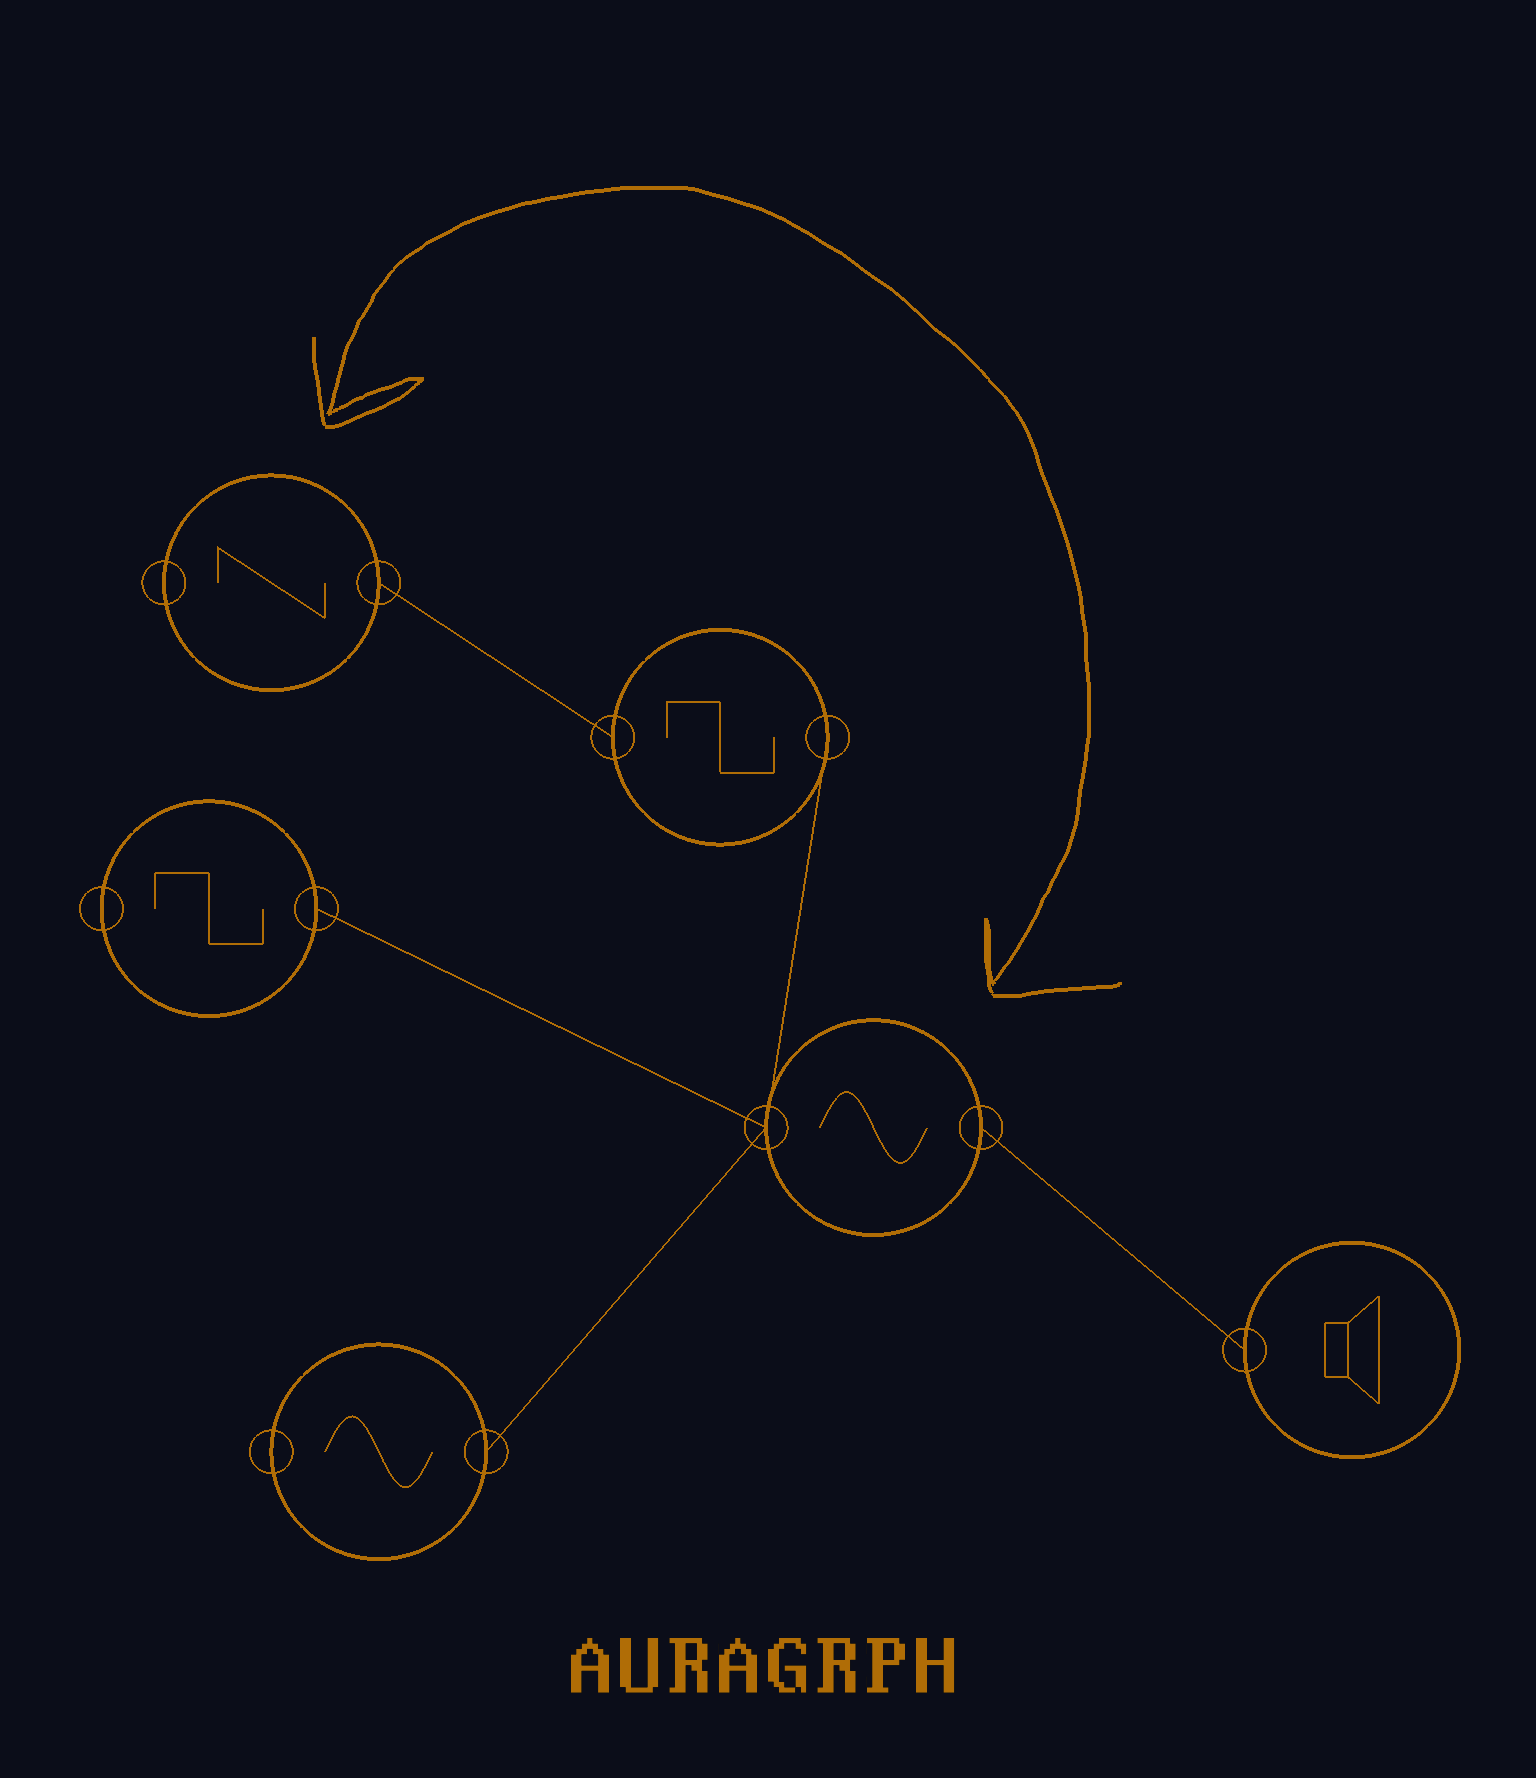
\includegraphics[width=0.45\textwidth]{figures/patch.png}
	\caption{A full Auraglyph patch.}
	\label{fig:patch}
\end{figure}

The basic environment of Auraglyph is an open, scrollable canvas in which the user freely draws. 
Using a variety of pen strokes, a user creates interactive objects (such as unit generators, control rate processors, and input/output controls), sets parameters of these objects, and forms connections between them, collectively comprising a \emph{patch}. 
After a user completes a pen stroke (a single contour between touching the pen to the screen and lifting it off the screen), this stroke is matched against the set of base object glyphs available in the main canvas, via a machine learning-based handwriting recognizer (discussed in Section \ref{sec:HandwritingRecognition}). 
The main canvas objects whose glyphs can be matched include an audio rate processor (unit generator), control rate processor, input, or output (see Section \ref{sec:BaseGlyphs}). 
If the stroke matches an available glyph, the user's stroke is replaced by the actual object. 
Unmatched strokes remain on the canvas, allowing the user to embellish the canvas with freehand drawings. 

Tapping and holding an object will open up a list of parameters for that object (Figure \ref{fig:editor}). 
Selecting a parameter from this list opens a control into which writing a number will set the value. 
This value can then be accepted or discarded, or the user can cancel setting the parameter. 

Every base object may have an input node, an output node, or both, visualized by small circles on the perimeter of the object. 
Tapping a node will highlight it, and by drawing a stroke from an input node to an output node, or vice-versa, the user forms a connection between those two objects. 
Most objects only have one output source, but an object input node may have several destinations with that object (e.g. frequency, amplitude, or phase of a given oscillator). 
In such cases, a pop-up menu appears from the input node to display the options a user may have for input destination. 

Objects and drawings can be moved around on the canvas by touching and dragging them, a familiar gesture in the touchscreen software ecosystem. 
While dragging an object, moving the pen over a delete icon in the corner of the screen will remove that object, along with destroying any connections between it and other objects. 
Connections can be removed by grabbing them with a touch and then dragging them until they ``break."

\begin{figure}[h]
	\centering
		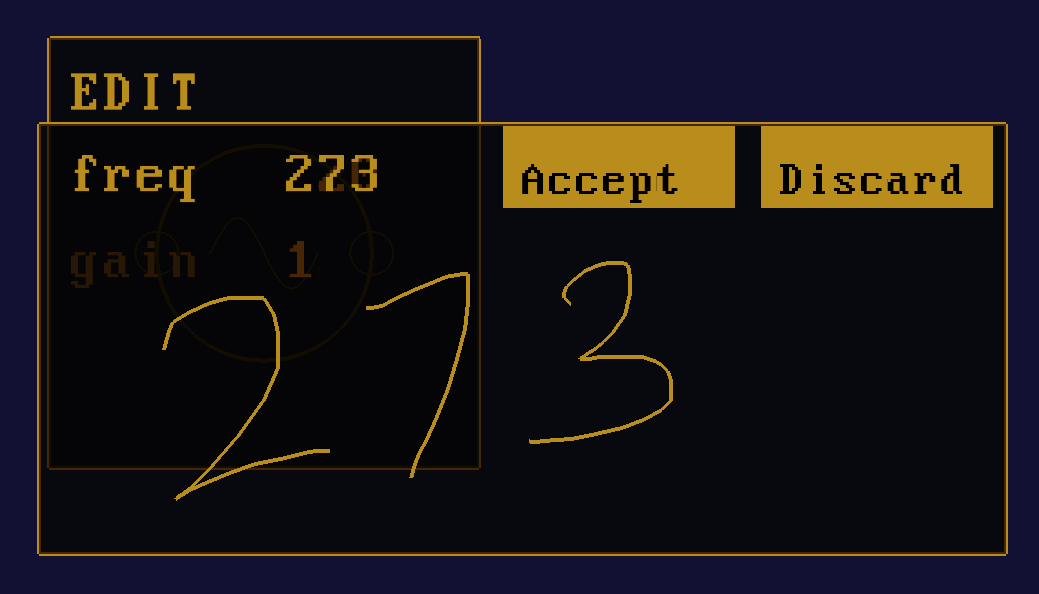
\includegraphics[width=0.45\textwidth]{figures/editor.png}
	\caption{Modifying the ``freq'' parameter of a unit generator with handwritten numeric input.}
	\label{fig:editor}
\end{figure}

\subsection{Objects}
\label{sec:BaseGlyphs}

Four base objects comprise the set of objects that can be drawn to the main canvas: audio-rate processors (unit generators; represented by a circle), control-rate processors (represented by a square), inputs (a downward-pointing triangle), and outputs (an upward triangle) (Figure \ref{fig:baseObjects}). 
Unit generators currently available include basic oscillators (sine, sawtooth, square, and triangle waves, plus hand-drawn wavetables), envelopes (linear and ADSR), filters (resonant low-pass/high-pass/band-pass, parametric EQ, or hand-drawn transfer function), and a reverberator. 
Control-rate processors include timers, discrete time-step sequencers, and hand-drawn parameter control curves. 
Inputs consist of on-screen keyboard controllers, graphical sliders, and buttons. 
Outputs comprise of numeric displays and binary ``LED'' indicators.  

After creating a base object, a drawing area and menu open to allow the user to select an object sub-type. 
In some cases, a glyph for the sub-type can be directly drawn by the user to select that object. 
For example, basic oscillators and filter types lend themselves to simple glyph patterns. 
A user can create a sine wave oscillator by simply drawing a circle (to create a unit generator object) and then drawing a sine wave within it. 
However some object sub-types do not have straightforward glyph mnemonics, for example a sequencer object or a reverberator. 
For such objects, a list of items to select from is provided in a menu. 
For completeness objects that do have corresponding glyphs are also listed in this menu. 

\begin{figure}[h]
	\centering
		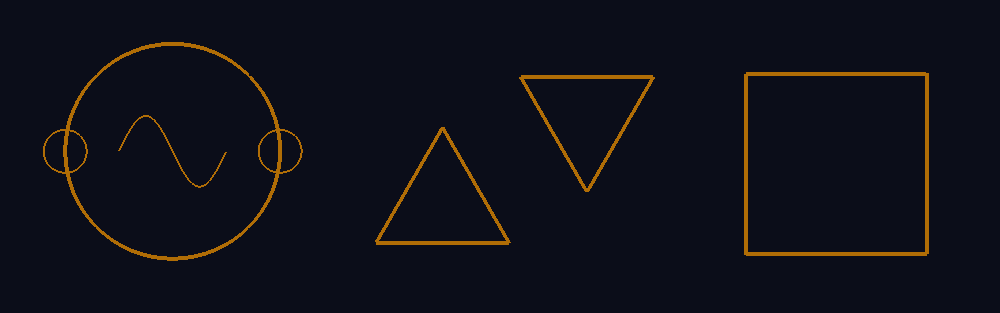
\includegraphics[width=0.45\textwidth]{figures/baseobjects.png}
	\caption{Base objects (left to right): unit generator, output, input, control-rate processor.}
	\label{fig:baseObjects}
\end{figure}

\subsection{Handwriting Recognition}
\label{sec:HandwritingRecognition}

The concepts presented herein are generally invariant to the underlying algorithms and framework for handwriting recognition, but these topics merit discussion with regards to our own implementation in Auraglyph. 
The underlying handwriting recognition engine of Auraglyph is LipiTk~\cite{madhvanath2007lipitk}, a comprehensive open-source project for handwriting recognition research. 
The default configuration of LipiTk uses dynamic time warping (DTW)~\cite{niels2005using} and nearest-neighbor classification (k-NN) to match pen strokes to a pre-existing training set of possible figures. 
The result of this procedure is one or more ``most likely'' matches along with confidence ratings for each match. 
We have found the speed and accuracy of LipiTk in this configuration to be satisfactory for real-time usage, though a slight, noticeable delay exists between finishing a stroke and the successful recognition of that stroke. 

The recognition algorithms underlying LipiTk must be seeded with a set of ``training examples'' for each possible figure to be matched. 
This training set is typically created in advance by having test users draw each figure into a specialized training program, which then serializes the salient features of the figures into a database. 
In our experience, LipiTk's recognition accuracy is highly linked to the quality and diversity of the training set. 
For instance, in one case, one version of our training set, seeded solely by right-handed users, suffered significantly reduced accuracy when being used by a left-handed user. 
A comprehensive training set would need to encompass strokes from a variety of individuals of varying handedness and writing style. 
Interestingly, though, LipiTk's algorithms are able to adapt dynamically to new training examples -- one might the recognizer gradually adjusting to a particular user's handwriting eccentricities over time, forming an organically personalized software interaction. 
Auraglyph takes advantage of this feature to a small degree, allowing a user to add new training strokes via a complementary training interface. 

%(iOS integration?)
\section{Conclusions}
\label{sec:Conclusions}

While successful in replacing the keyboard as a textual/numeric input device, touchscreen stylus input also affords a broader set of interactions apt for computer music. 
We have developed a software application for the iPad, Auraglyph, which leverages these principles into an interactive music environment. 
While this system has fulfilled the goals of expressivity and versatility, we believe this conceptual framework affords many more opportunities for computer music. 
Traditional music notation, extended mathematical formulae, and even Turing-complete programming code could conceivable be written out with a stylus. 
We believe that this is only the beginning for handwritten computer music. 

%\end{document}  % This is where a 'short' article might terminate

%
% The following two commands are all you need in the
% initial runs of your .tex file to
% produce the bibliography for the citations in your paper.
\bibliographystyle{abbrv}
\bibliography{auraglyph-nime2014}  % sigproc.bib is the name of the Bibliography in this case
% You must have a proper ".bib" file
%  and remember to run:
% latex bibtex latex latex
% to resolve all references
%
% ACM needs 'a single self-contained file'!
%

%\balancecolumns 

% That's all folks!
\end{document}
